\documentclass[tikz,border=5pt]{standalone}
\usepackage{tikz}
\usetikzlibrary{calc}

\begin{document}
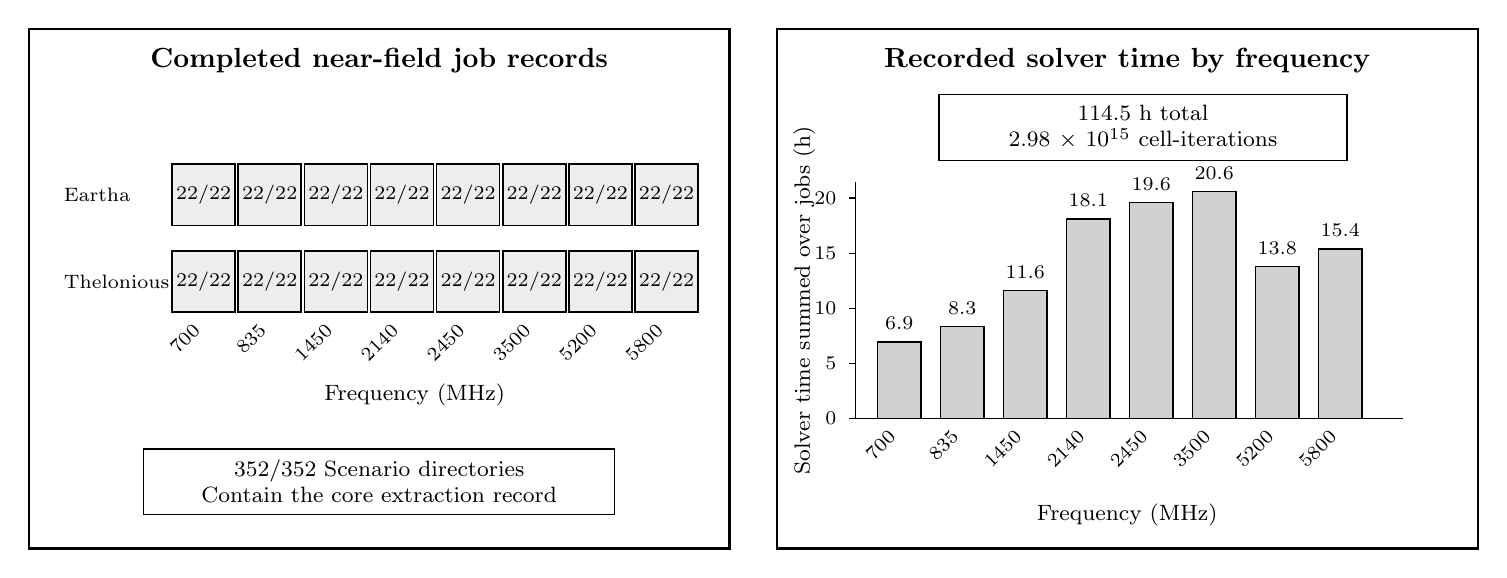
\begin{tikzpicture}[font=\rmfamily\small]
  \draw[line width=0.8pt] (0,0) rectangle (8.9,6.6);
  \node[font=\rmfamily\bfseries] at (4.45,6.20) {Completed near-field job records};

  \node[font=\rmfamily\scriptsize, anchor=west] at (0.32,4.49) {Eartha};
  \node[font=\rmfamily\scriptsize, anchor=west] at (0.32,3.39) {Thelonious};

  \foreach \x/\freq in {1.82/700,2.66/835,3.50/1450,4.34/2140,5.18/2450,6.02/3500,6.86/5200,7.70/5800} {
    \draw[fill=black!7, line width=0.55pt] (\x,4.10) rectangle ++(0.80,0.78);
    \draw[fill=black!7, line width=0.55pt] (\x,3.00) rectangle ++(0.80,0.78);
    \node[font=\rmfamily\scriptsize] at ($(\x,4.10)+(0.40,0.39)$) {22/22};
    \node[font=\rmfamily\scriptsize] at ($(\x,3.00)+(0.40,0.39)$) {22/22};
    \node[font=\rmfamily\scriptsize, rotate=45, anchor=east] at ($(\x,2.90)+(0.40,0)$) {\freq};
  }
  \node[font=\rmfamily\footnotesize] at (4.90,1.95) {Frequency (MHz)};
  \node[draw=black, rectangle, align=center, font=\rmfamily\footnotesize,
        text width=5.7cm, inner sep=4pt] at (4.45,0.85)
        {352/352 Scenario directories\\Contain the core extraction record};

  \draw[line width=0.8pt] (9.5,0) rectangle (18.4,6.6);
  \node[font=\rmfamily\bfseries] at (13.95,6.20) {Recorded solver time by frequency};

  \draw[line width=0.65pt] (10.5,1.65) -- (17.45,1.65);
  \draw[line width=0.65pt] (10.5,1.65) -- (10.5,4.65);
  \foreach \y/\lab in {1.65/0,2.35/5,3.05/10,3.75/15,4.45/20} {
    \draw[line width=0.45pt] (10.42,\y) -- (10.5,\y);
    \node[font=\rmfamily\scriptsize, anchor=east] at (10.38,\y) {\lab};
  }
  \node[font=\rmfamily\footnotesize, rotate=90] at (9.85,3.15) {Solver time summed over jobs (h)};

  \foreach \x/\height/\freq/\hours in {
    10.78/0.973/700/6.9,
    11.58/1.167/835/8.3,
    12.38/1.625/1450/11.6,
    13.18/2.534/2140/18.1,
    13.98/2.744/2450/19.6,
    14.78/2.884/3500/20.6,
    15.58/1.932/5200/13.8,
    16.38/2.156/5800/15.4} {
    \draw[fill=black!18, line width=0.6pt] (\x,1.65) rectangle ++(0.55,\height);
    \node[font=\rmfamily\scriptsize, anchor=south] at ($(\x,1.65)+(0.275,\height+0.03)$) {\hours};
    \node[font=\rmfamily\scriptsize, rotate=45, anchor=east] at ($(\x,1.55)+(0.275,0)$) {\freq};
  }
  \node[font=\rmfamily\footnotesize] at (13.95,0.42) {Frequency (MHz)};
  \node[draw=black, rectangle, align=center, font=\rmfamily\footnotesize,
        text width=4.9cm, inner sep=4pt] at (14.15,5.35)
        {114.5 h total\\$2.98\times10^{15}$ cell-iterations};
\end{tikzpicture}
\end{document}
